\chapter{Grundlagen} \label{grundlagen}
 
 In diesem Kapitel werden die  wichtigsten Grundlagen erklärt, die zum Verständnis dieser Arbeit notwendig sind. 
 Als erstes werden die \emph{mathematischen Notationen} der verwendeten Symbole und Operationen, insbesondere Matrixoperatoren, eingeführt. 
 Daraufhin wird auf das Thema \emph{Beleuchtung} eingegangen und erklärt wie sich die Beleuchtung, die auf eine Szene einfällt, mathematisch darstellen lässt.
 Es wird das Konzept des \emph{Dynamikbereichs} erklärt, mit dem das Kontrastverhältnis einer Beleuchtungen sowie von Lichterzeugenden und -aufnehmenden Geräten beschrieben werden kann.
 Desweiteren wird das \emph{Pinhole-Modell} vorgestellt, mit dem Kameras geometrisch modelliert werden können, sodass mit ihnen eine \emph{Positionsbestimmung} möglich ist. 
 Zuletzt werden die Bildschirmtechnologien betrachtet. die in gängigen portablen Geräten zu finden sind, und gezeigt worin die Unterschiede im Hinblick auf die Lichterzeugung liegen.
 
 
%%%%%%%%%%%%%%%%%%%%%%%%%%%%%%%%%%%%%%%%%%%%%%%%%%%%%%%%%%%%%%%%
  
\section{Notationen} \label{notation}

 Diese Arbeit hält sich an die üblichen mathematischen Konventionen:
 Skalare Werte und Funktionen werden mit Kleinbuchstaben bezeichnet, für Vektoren und vektorwertige Funktionen wird ein Pfeil übergestellt. 
 Matrizen, wozu auch Rasterbilder gehören, werden mit Großbuchstaben bezeichnet. 
 Ein Element einer Matrix, also auch ein Pixel eines Bildes, wird mit ganzzahligen Koordinaten $(x,y)$ adressiert, wobei $(0,0)$ das Element in der linken oberen Ecke bezeichnet.
% Das dreidimensionale Weltkoordinatensystem ist rechtshändig; Koordinaten darin werden mit (x,y,z) bezeichnet.
 
 In Tabelle \ref{operationen}  sind alle verwendeten Matrix- und Vektoroperationen aufgeführt. 
 Damit soll klargestellt werden, bei welchen Operationen es sich um Elementweise Operationen handelt, da sie bei der Behandlung von Bildern häufig benötigt werden.

 \begin{table}[H]
  \begin{tabular}{cl}
   $ aB $ 			& Skalarmultiplikation \\ 
   $AB $ 			& Matrixmultiplikation \\
   $A\vec{b}$ 			& Matrix-Vektor Multiplikation \\
   $A \cdot B $ 		& Elementweise Multiplikation \\ 
   $A / B $ 			& Elementweise Division \\ 
%   $\vec{a} \times \vec{b}$   	& Kreuzprodukt \\
   $A(i,j) $ 			& $i$-tes Element von links in der $j$-ten Zeile von oben \\ 
   $A \leq B $           	& Elementweiser Vergleich: muss für alle Elemente gelten\\
   $A=n$			& Alle Elemente setzen oder vergleichen\\
%   $ \lVert A \rVert $ 		& Euklidische Distanz ($L_2$ Norm)\\
   $\max{(A)}\ ,\ \ \min{(A)}$	& Das größte / kleinste Element \\
%   $\max{(A,B)} \ \ ,\ \ \min{(A,B)}$	& Erzeugt Matrix mit den größten / kleinsten Elementen. \\
   %$\lfloor A \rfloor \ \ ,\ \  \lceil A \rceil$ & Elementweises Ab- und Aufrunden zum Ganzahlwert (\emph{floor} und  \emph{ceil}) \\
   %$\lbrack A  \rbrack _{l}^{u} $ & Elementweise Wertbegrenzung zwischen $l$ und $u$ ( \emph{clamp}) \\
  % $\lfloor A \rfloor \ \ ,\ \  \lceil A \rceil$ & Elementweises Ab- und Aufrunden zum Ganzahlwert (\emph{floor} und  \emph{ceil}) \\
  % $\lbrack A  \rbrack _{l}^{u} $ & Elementweise Wertbegrenzung zwischen $l$ und $u$ ( \emph{clamp}) \\
%   $\measuredangle(\vec{a},\vec{b})$ & Winkel zwischen zwei Vektoren, in Radiant \\
   
   \caption[Matrix- und Vektoroperationen]{\label{operationen} Notationen der verwendeten Matrixoperationen. Alle elementweise arbeitende Operationen und Funktionen gelten auch für Vektoren.}

  \end{tabular}
 \end{table}


%%%%%%%%%%%%%%%%%%%%%%%%%%%%%%%%%%%%%%%%%%%%%%%%%%%%%%%%%%%%%%%%

 \section{Licht und Beleuchtung} \label{light}
   
    In jeder realen Umgebung befinden sich Lichtquellen, die dafür sorgen, dass sie durch und durch von Licht durchdrungen ist.
    Eine kleine Szene die sich darin befindet, wie beispielsweise ein einzelnes Objekt, wird durch das Licht, das von der umgebenden Materie ausgeht, rundum beleuchtet.
    Wenn die Szene selbst keine Lichtquellen beinhaltet so kann man die Umgebung als die einzige Quelle betrachten.
    Unter der Annahme, dass der Ursprung des Lichts das die Szene erreicht, unendlich weit von ihr entfernt ist, ist eine mathematische Beschreibung der einfallenden Beleuchtung einfach möglich:
    Das Licht, das in einem Punkt der Szene eingeht, kann mit einer Funktion
    
   \begin{equation}
     l_{dist}(\phi, \theta)
    \label{eq:distant_light}
   \end{equation}
 
    beschrieben werden, welche die aus der Richtung $(\phi,\theta)$  eingehende Strahldichte beschreibt.

    Dieser Sachverhalt wird in dieser Arbeit als ``distante Beleuchtung''  (engl: ``distant illumination'') bezeichnet.
    Eine distante Beleuchtung kann man mit unendlich weit entfernten Punktlichtquellen modellieren, die kugelförmig rund um die Szene angeordnet sind.
    In der Praxis ist eine distante Beleuchtung natürlich nicht realisierbar.
    Ist die Entfernung der Lichtquellen jedoch deutlich größer als der Radius der Szene (Abbildung \ref{fig:distant_light}), so kann eine distante Beleuchtung approximiert werden. 
    Beispielsweise weicht bei einem Verhältnis von $ r_l / r_s > 10$ die Richtung der einfallenden Lichtstrahlen um nicht mehr als atan$(0.1) \approx 5.71^\circ$ ab. 
    Vergrößert man den Abstand oder reduziert den Szeneradius, so verbessert sich die Approximation entsprechend.

    Hier sei anzumerken dass mit dem Begriff ``Strahldichte'' in dieser Arbeit ausschließlich \emph{relative} Strahldichte gemeint ist.
    Sie ist proportional zur absoluten Strahldichte, hängt jedoch mit ihr über einen unbekannten Faktor zusammen.
    Aufgrund der linearen Eigenschaft von Lichttransport darf die relative Strahldichte in allen linearen Rechenoperationen verwendet werden, solange kein direkter Bezug zu absoluten Messwerten bestehen muss.
    

   \begin{figure}[h]
    \centering
    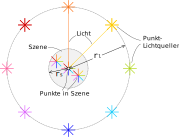
\includegraphics[width=0.6\textwidth]{../graphics/grundlagen/distant_light.svg}
    \caption[Beleuchtung durch weit entfernte Punktlichtquellen]{ 
     Eine Szene mit dem Radius  $r_s$ wird von mehreren Punktlichtquellen beleuchtet, die sich in einem Abstand von $r_l$ zum Szenenmittelpunkt befinden. 
     Wenn der Quotient  $r_l / r_s $ groß genug ist, so kann davon ausgegangen werden, dass in allen Punkten der Szene aus jeder Richtung das selbe Licht einfällt.
     Damit lässt sich eine Approximation der einfallenden Beleuchtung mit Gleichung \ref{eq:distant_light} darstellen.
     
     }   
 \label{fig:distant_light}
   \end{figure}
  
   Das Prinzip der distanten Beleuchtung hat zahlreiche Anwendungen in der Computergrafik und anderen dazu verwandten Gebieten.
   Im Folgenden werden zwei davon vorgestellt, die im Zusammenhang zu dieser Arbeit stehen.
 

%%%%%%%%%%%%%%%%%%%%%%%%%%%%%%%%%%%%%%%%%%%%%%%%%%%%%%%%% 

 \subsection{Enviroment-Mapping} \label{envmaps}

   Das Environment-Mapping-Verfahren und die dabei verwendeten Environment-Maps wurden im Jahr 1976 von Blinn und Newell vorgestellt \cite{Blinn_1976}.
   Ihr Ziel dabei war das Rendern spiegelnder Objekte mit vorwiegend konvexen Oberflächen, was mit den Methoden dieser Zeit noch nicht möglich war.
    Spiegelnde Oberflächen reflektieren die gesamte Umgebung, inklusive allen anderen Objekte die sich darin befinden, weshalb Strahlverfolgenden Verfahren wie zum Beispiel Raytracing eingesetzt werden müssen. 
   Mit dem Environment-Mapping haben sie eine Methode vorgestellt, die ohne großen Aufwand verblüffend realistische Ergebnisse erzielt. 
   Sie nehmen dabei eine distante Beleuchtung an und speichern das in die Szene einfallende Licht in einer Environment-Map.
   Dabei handelt es sich um eine gewöhnliche zweidimensionale Textur, wobei eine der Dimensionen für die Darstellung des Polarwinkels $\phi$  und eine für den Azimutalwinkel $\theta$ der Einfallsrichtung verwendet wird.
   Die Intensität des Lichts, das von jedem Punkt des Objekts zur Kamera reflektiert wird, kann dann ganz einfach berechnet werden: 
   Anhand der Oberflächennormale an einem Punkt lässt sich der Reflexionsvektor berechnen, womit die Richtung des einfallenden Lichstrahls bekannt ist. 
   Seine Strahldichte kann dann direkt durch Nachschlagen des zugehörigen Pixels in der Environment-Map ermittelt werden.
   Damit lassen sich mit sehr geringem Aufwand realistische Ergebnisse erzielen, weshalb Environment-Mapping auch heute noch häufig in der Computergrafik eingesetzt wird. 
   
   Die von Blinn und Newell verwendete winkelparametrisierte Environment-Map besitzt einige Nachteile, wie beispielsweise eine stark ungleichmäßige Auflösung und rechenaufwändige Winkeloperationen, weshalb im Laufe der Zeit praxistauglichere Parametrisierungen entwickelt wurden.
   Eine häufig anzutreffende Darstellungsform ist die \emph{Cube-Map} \cite{Akenine_2011}. 
   Man kann sie sich als ein Würfel aus sechs Texturen vorstellen, der rund um eine Szene aufgespannt ist (Abbildung \ref{fig:cubemap}). 
   Die Pixel der Texturen speichern dabei die Strahldichte eines Lichstrahls, und ihre Koordinaten auf der Textur geben die Lichtrichtung an.
   
 
   \begin{figure}[h]
    \centering
    \begin{tabular}{c}
     \includegraphics[width=0.4\textwidth]{../graphics/grundlagen/cubemap.svg}
     \\
     \includegraphics[width=\textwidth]{../graphics/grundlagen/ennis_cubemap.png}
    \end{tabular}
    \caption[Aufbau einer Cube-Map]{
    
     Oben: Eine Cube-Map besteht aus sechs Texturen, die man sich rund um eine Szene angeordnet vorstellen kann.
     Ein Pixel speichert dabei die in den Ursprung einfallende Strahldichte $l_i$, und seine Koordinaten bestimmen die Richtung.
     Unten: Die sechs Texturen einer Cube-Map, nebeneinander dargestellt. Sie wurden anhand der  ``Ennis-Brown House''-Environment-Map aus der Debevec High-Res Light Probe Gallery \cite{lightprobe_gallery} berechnet.
      } 
    \label{fig:cubemap}
   \end{figure}
   

%%%%%%%%%%%%%%%%%%%%%%%%%%%%%%%%%%%%%%%%

   \subsection{Light-Stages} \label{lightstages}

   Eine \emph{Light-Stage} kann man als eine reale Implementierung einer Environment-Map ansehen.
   In den meisten Fällen besteht sie aus zahlreichen, einzeln steuerbaren Lampen, die kugelförmig rund um eine Szene angeordnet sind (Abbildung \ref{fig:lightstage}). 
    Wenn Szenendurchmesser und Lichtquellenabstand so gewählt werden, dass die Annahme einer distanten Beleuchtung erfüllt wird, dann kann man die Lampen als Punktlichtquellen ansehen, ihre Helligkeit durch Abtasten einer Environment-Map berechnen und eine einfallende Beleuchtung erzeugen.
    Die Auflösung dieser Beleuchtung ist jedoch stark eingeschränkt, da die Lampen nicht beliebig weit entfernt positioniert oder beliebig klein gebaut werden können.
    Aus diesem Grund eignen sich Light-Stages nicht zur Beleuchtung spiegelnder Objekte, denn man würde die einzelnen Lampen auf der Oberfläche erkennen können.
    Für diffuse Szenen sind sie hingegen sehr gut geeignet, weshalb sie in der Forschung zahlreiche Anwendungen haben (siehe Abschnitt \ref{rel:lightstages})

   \begin{figure}[h]
    \centering
    \includegraphics[width=0.6\textwidth]{../graphics/grundlagen/debevec_lightstage.png}
    \caption[Eine Light-Stage]{Die ``Light-Stage 3'' von Debevec et al. erzeugt eine einfallende Beleuchtung mit Hilfe zahlreicher computergesteuerter Lampen (Bildquelle: \cite{Debevec_2002}) }
    \label{fig:lightstage}
   \end{figure}

 
%%%%%%%%%%%%%%%%%%%%%%%%%%%%%%%%%%%%%%%%

  \section{Dynamikbereich} \label{dynamikbereich}
   
    Der \emph{Dynamikbereich} (auch: Kontrastverhältnis) beschreibt das Verhältnis zwischen dem größten und dem kleinsten Wert \emph{größer $0$}, welches ein Gerät oder System speichern, darstellen, aufnehmen oder allgemein handhaben kann. 
    Er kann, je nach Anwendungsgebiet, auf jede beliebige messbare technische Größen (Licht, Schalldruck, Strahlung usw.) bezogen werden.
    Für diese Arbeit wird der Dynamikbereich $R$ über die relative Strahldichte definiert und lautet 
    \begin{equation}
      %R = \frac{\text{größtmögliche Strahldichte}}{\text{kleinstmögliche Strahldichte}}
      R = \frac{l_{max}}{l_{min}} \hspace{10mm} \text{wobei} \ \ \  l_{min} > 0
     \label{eq:dynamic_range} 
   \end{equation} 
    wobei  $l_{max}$ und $l_{min}$ die kleinste beziehungsweise die größte Strahldichte bezeichnet.
   Damit lässt sich der Dynamikbereich einer Umgebungsbeleuchtung oder einer Aufnahme berechnen.

   Soll jedoch der Dynamikbereich eines Bildschirms oder einer Kamera ermittelt werden, so muss der kleinste beziehungsweise größte Wert verwendet werden, der mit\emph{jedem} Pixel darstellbar ist.
    Ein Beispiel: Ein Bildschirm, bei dem jedes Pixel in der Lage ist $l_{max}=100.0$ und $l_{min}=1.0$ zu erzeugen, hat einen Dynamikbereich von $R=100$, auch geschrieben als $100:1$

    Es sei anzumerken dass das Kontrastverhältnis eines Flachbildschirms vom Hersteller üblicherweise über die Leuchtdichte, und nicht die Strahldichte angegeben wird. 
    Da der Bildschirm in dieser Arbeit jedoch nicht von einem Menschen betrachtet wird, sondern zum Erzeugen einer Strahldichteverteilung in einem Punkt verwendet wird, ist die Definition in Gleichung \ref{eq:dynamic_range} zu verwenden.
    $R$ kann darum nicht mit den Herstellerangaben verglichen werden.


%kameras    
    Der Dynamikbereich spielt eine wichtige Rolle in der Fotografie: Die Strahldichte in einer realen Szene kann um mehr als 10 Größenordnungen variieren \cite{Reinhard_2005} - deutlich mehr als man mit einer Kamera in einem Bild aufnehmen kann.
    Man spricht hier jeweils von High Dynamic Range ("HDR") und Low Dynamic Range ("LDR"), wobei Digitalkameras und Bildschirme zu LDR gezählt werden, und eine reale, Sonnenbeleuchtete Szene dagegen zu HDR  \cite{Reinhard_2005}.

%bildschirme
 
    Das Menschliche Auge kommt sehr gut mit dem großen Dynamikbereich einer natürlichen Szene zurecht, und kann bis zu 5 Größenordnungen gleichzeitig wahrnehmen \cite{Reinhard_2005}.
    Damit auf einem Bildschirm eine echte Szene realistisch dargestellt werden kann, muss er also auch einen entsprechend hohes Kontrastverhältnis besitzen.
    In der Praxis ist dies nicht der Fall: Nahezu alle Bildschirme sind LDR, da für ein HDR-Display ein deutlich höherer technischer Aufwand erforderlich ist. 
    HDR-Bildschirme und HDR-Kameras sind aktuell noch Forschungsgegenstand und nicht im Konsumerbereich anzutreffen.

    Im Folgenden werden die aktuell verbreiteten Bildschirmtechnologien vorgestellt, und die Unterschiede im Hinblick auf die Erzeugung einer (HDR-) Beleuchtung dargelegt.
     
%%%%%%%%%%%%%%%%%%%%%%%%%%%%%%
 
 \section{Bildschirme} \label{bildschirme}
    
   %Bildschirmtechnologien%
%LC
    Die Entwicklung von Flachbildschirmen ist immer noch in vollem Gange und es ist noch lange kein Ende in Sicht.
    Die wichtigste Technologie stellt dabei seit langem der Flüssigkristall dar, der die Basis für alle LCD-Bildschirme (LCD, TFT) bildet.
    Ein Flüssigkristallbildschirm nutzt den Effekt der Polarisation, womit die Lichtmenge geregelt werden kann die ein einzelnes Pixel transmittiert.
    Das Licht, das von diesen Bildschirmen ausgeht, wird von einer gemeinsamen Hintergrundbeleuchtung erzeugt und durch die mit einem Farbfilter versehenen Pixel moduliert.
    Diese Hintergrundbeleuchtung befindet sich in der Regel im Rahmen des Bildschirms und wird durch einen Lichtleiter über die gesamte Bildschirmfläche verteilt. 
    Sie ist, besonders bei einer kompakten Bauweise in mobilen Geräten, sehr unregelmäßig und variiert über die Oberfläche.

    Der Dynamikbereich eines Bildschirms wird zum Einen von der maximalen Helligkeit der Hintergundbeleuchtung, und zum Anderen von dem Regelbereich der Pixel limitiert. 
    LCD-Bildschirme haben die intrinsische Eigenschaft, dass ein Pixel nicht vollständig auf ``undurchlässig'' geschaltet werden kann - es geht zwangsläufig immer Licht von den Pixeln aus. 
    Das sorgt für den hohen Schwarzwert der für diese Bildschirme typisch ist.

    Desweiteren sind LCD-Bildschirme stark Blickwinkelabhängig - die maximale Strahldichte, aber auch das Ansprechverhalten des Bildschirms, hängt maßgeblich von der Richtung ab, unter der das Licht die Oberfläche verlässt.
    Bedingt durch die Konstruktion der Pixel ist dieser Effekt besonders bei älteren und kostengünstigen Bildschirmen ausgeprägt (TN-Technologie), konnte jedoch durch andere Bauweisen verbessert werden (IPS-Technologie).
    Abbildung \ref{fig:angular_effects} zeigt diesen Effekt anhand eines TN-Bildschirms, der aus zwei unterschiedlichen Blickwinkel fotografiert wurde.

  \begin{figure}[H]
    \centering
    \begin{tabular}{cc}
      \includegraphics[width=0.4\textwidth]{../graphics/grundlagen/lenovo_angle_v-10.png}
    & 
      \includegraphics[width=0.4\textwidth]{../graphics/grundlagen/lenovo_angle_v+10.png}
    \\  
    a) $10^\circ$ von oben & b) $10^\circ$ von unten \\
    \end{tabular}
    \caption[Blickwinkelabhängigkeit bei einem TN-Bildschirm]{Ein 3x3x3 Bit Unterraum des möglichen 8x8x8-Bit Farbraums wurde auf einem  TN-Bildschirm dargestellt, und unter zwei verschiedenen Blickwinkeln aus 2.5 Meter Entfernung fotografiert. 
   Es ist gut zu sehen dass sich das Ansprechverhalten des Bildschirms sich dabei verändert.   }
    \label{fig:angular_effects}
   \end{figure}

 
% LED   
    Eine relativ neue Technologie, die diese Probleme nicht besitzt, ist der LED-Bildschirm (``AMOLED'', ``OLED''), der auf einem ganz anderen Ansatz basiert:
    Die Pixel werden dabei durch einzelne Leuchtdioden (``LED'') bestehen also aus diskreten Lichtquellen. 
    Damit ist es möglich, einen Pixel komplett auszuschalten, weshalb diese Bildschirme einen hervorragenden Schwarzwert und somit eine größeres Kontrastverhältnis als LCD-Bildschirme besitzen.
    Zudem ist das abgestrahlte Licht weitaus weniger Richtungsabhängig - ein dargestelltes Bild sieht von jeder Richtung gleich aus.

    Zu den Nachteilen dieser Technologie gehört zum Einen der hohe Preis, weshalb sie vorwiegend in kleinen portablen Geräten wie Smartphones oder Tablets zu finden sind. 
    Zum Anderen leiden sie unter einer begrenzten Lebensdauer:
    Insbesondere bei organischen LED-Bildschirmen (AMOLED) degenieren die Pixel in Abhängigkeit der Nutzungsdauer und abgestrahlter Lichtleistung und ihre Lichtleistung reduziert sich.
    Abbildung \ref{fig:amoled_usage} zeigt diesen Effekt, wie er bei der radiometrischen Vermessung eines AMOLED-Bildschirms beobachtet werden konnte.

  \begin{figure}[H]
    \centering
    \includegraphics[width=0.7\textwidth]{../graphics/grundlagen/s4_usage_map.png}
    \caption[Abgenutzte Pixel eines LED-Bildschirms]{ Die senkrecht zur Oberfläche gemessene, relative Strahldichte bei einem Samsung S4 Smartphone Bildschirm (AMOLED-Technologie).
   Man kann deutlich erkennen, dass auf der linken Seite, insbesondere im unteren Bereich, die Lichtleistung reduziert ist.  
   Dort wurden über einen längeren Zeitraum weiße, rechteckige Flächen mit maximaler Intensität angezeigt, wodurch sich die Pixel ``abgenutzt'' haben. }
    \label{fig:amoled_usage}
   \end{figure}


 \section{Kameras} \label{pinhole}
   
   Eine Kamera sammelt Lichstrahlen ein und bildet sie auf eine Ebene ab.
   Bei einer \emph{idealen Kamera} geschieht dies durch eine punktförmige Blende, durch die das Licht fällt und auf einen planen Sensor abgebildet wird (Abbildung \ref{fig:cam_model}). 
   Durch die unendlich kleine Blende, die dabei angenommen wird, werden vom Sensor im Grunde genommen einzelne Lichtstrahlen wahrgenommen  - der Sensor misst also die Strahldichte, die durch die Punktblende verläuft.
   Dieses Modell wird auch als \emph{Pinhole-Modell} bezeichnet, und kann zur geometrischen Modellierung von echten Kameras verwendet werden.   
   Der Sensor der Kamera besitzt dabei ein gewisses Ansprechverhalten das beschreibt, wie die aufgenommene Strahldichte in einen digitalen Ausgabewert umgesetzt wird. 

   Echte Kameras verwenden natürlich keine punktförmige Blende, sondern nutzen ein Linsensystem. 
   Es erfüllt dabei allerdings die selbe Funktion, weshalb auch sie mit dem Pinhole-Modell beschrieben werden können.
   Im Unterschied zur idealen Kamera treten bei einer echten Kamera  weitere, meist unerwünschte Effekte auf, wie beispielsweise Verzerrungen durch die Linsen. 
   Sie müssen separat betrachtet und korrigiert werden, und werden vom Pinhole-Modell nicht erfasst.
   
   \begin{figure}[H]
    \centering
    \includegraphics[width=0.6\textwidth]{../graphics/grundlagen/pinhole.svg}
    \caption[Funktionsweise einer idealen Kamera]{Die ideale Kamera besitzt eine punktförmige Blende, durch welche die Lichtstrahlen einer Szene auf eine Sensorebene abgebildet wird. Dieser Prozess kann mit einer perspektivischen Projektion modelliert werden.}
    \label{fig:cam_model}
   \end{figure}

  Mathematisch lässt sich die Abbildung, die in einer idealen Kamera geschieht, als eine Zentralperspektivische Projektion (engl ``perspective projection'') mit einer $3\times3$ Matrix beschreiben \cite{camera_matrix}.
   Diese Matrix  $C$ wird als auch als die \emph{intrinsischen Parameter} der Kamera bezeichnet, und beschreibt, wie das Licht aus der Szene auf die einzelnen Sensorpixel abgebildet wird.
   Die Rotation ($3\times3$-Matrix $R$ ) und Translation (Vektor $\vec{t}$) der Kamera in der Welt werden mit einer $3\times4$ Transformationsmatrix  $D=[R|\vec{t}\;]$ erfasst, welche als die \emph{extrinsischen Parameter} bezeichnet wird.

   \begin{equation}
     s \begin{pmatrix}  u \\ v \\ 1 \end{pmatrix} =  C[R|\vec{t}\;]	 
     \begin{pmatrix}  x \\ y \\ z \\ 1  \end{pmatrix} = 
     \begin{pmatrix}  
         f_x & 0 & c_x \\ 
         0  & f_y & c_y \\ 
         0  & 0 & 1 \\ 
     \end{pmatrix}
     \begin{pmatrix}  
         r_{11} & r_{12} & r_{13} & t_1 \\ 
         r_{21} & r_{22} & r_{23} & t_2 \\ 
         r_{31} & r_{32} & r_{33} & t_3 \\ 
     \end{pmatrix}
     \begin{pmatrix}  x \\ y \\ z \\ 1  \end{pmatrix}
     \label{eq:pinhole}
   \end{equation}

   Die Matrix $C$ bildet einen Punkt der Szene, welcher die Koordinaten $(x,y,z)$ besitzt, auf ein Sensorpixel mit den Koordinaten $(u,v)$ ab. Sie werden dabei mit homogenen Koordiaten beschrieben.
   $C$ beinhaltet die geometrischen Eigenschaften der Kamera: $f_x$ und $f_y$ ist die Brennweite, ausgedrückt in Pixelkoordinaten, $c_x$ und $c_y$ ist der Punkt auf dem Sensor, durch den die optische Achse verläuft.
   
   Kennt man die intrinsischen Parameter einer Kamera, so bezeichnet man sie als \emph{geometrisch kalibriert}. 
   Damit ist es unter anderem möglich, anhand eines Eingabebildes die extrinsischen Parameter zu berechnen - eine kalibrierte Kamera kann also zur Positionsbestimmung eingesetzt werden.
   
 \subsection{Positionsberechnung mit Kameras} \label{pos_kameras}
   Anhand der Kameramatrix kann die Richtung des Lichtstrahls berechnet werden, der auf ein bestimmtes Sensorpixel fällt.
   Platziert man ein Muster mit einer bekannten Geometrie im Frustum der Kamera, so kann man es in der Aufnahme lokalisieren und anhand der Pixelpositionen die extrinsischen Parameter berechnen. 
   Kennt man die Position der Muster in der Welt, so ist auch die Rotation und Position der Kamera innerhalb der Welt berechenbar.

   \begin{figure}[H]
    \centering
    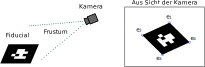
\includegraphics[width=0.7\textwidth]{../graphics/grundlagen/positionsbestimmung.svg}
    \caption[Positionsberechnung mit einer Kamera]{Positionsberechnung mit einer geometrisch kalibrierten Kamera: Im Frustum der Kamera befindet sich ein Muster (ein ``Fiducial''), dessen Geometrie und Lage im Raum bekannt ist. 
   Es wird im Kamerabild lokalisiert, und die Position der Eckpunkte  $e_1$-$e_4$ berechnet. Durch Anwendung des Pinhole-Modells (Gleichung \ref{eq:pinhole}) kann damit ein Gleichungssystem aufgestellt werden, mit dem nach den extrinsischen Parametern gelöst werden kann.}
    \label{fig:positionsbestimmung}
   \end{figure}

   Diese Verfahren wird gerne im Bereich Augmented Reality (``AR'') verwendet:
   Kennt man nämlich die extrinsischen Parameter der Kamera, so lässt sich damit ganz einfach ein dreidimensionales Objekt aus dem richtigen Blickwinkel rendern und in den Kamerastream überlagern.
 
   Eine freie Implementierung eines solchen AR-Systems ist die ARToolKit Library \cite{artoolkit}.
   Sie setzt simple schwarze Quadrate als Fiducials ein, die ganz einfach auf Papier ausgedruckt werden können.
   In der Mitte der Fiducials befindet sich ein Muster, durch das sie sich im Kamerastream auseinanderhalten und eindeutig identifizieren lassen. 
   Damit ist es möglich, nahezu beliebig viele Fiducials gleichzeitig zu verwenden.
   In dieser Arbeit wird ARToolKit zur Positionsberechnung verwendet, da nicht nur sehr schnell ist sondern auch zuverlässig mit einfachen  Webcams funktioniert und viele Fiducials gleichzeitig eingesetzt werden können. 

% vergleich
%   \subsection{Vollstaendiges Modell eines Bildschirmes}
%
%  Ein vollstaendiges radiometrische Modell eines Bildschirms leasst sich mit einer 8-Dimensionalen Funktion beschreiben. 
%
%  \begin{equation}
%   l \colon  \mathbb{R} \times \mathbb{R}^2 \times \mathbb{R}^2 \times \mathbb{N}^2  \rightarrow \mathbb{R}, \hspace{10mm}  l(\nu,x,y,\phi,\theta,B)
%  \label{complete_displaymodel}
%  \end{equation}
% 
%  Die kontinuierliche Funktion f beschreibt die spektrale Strahldichte der Frequenz $\nu$ die fuer ein gegebenen Framebuffer $B$ an einer Position $(x,y)$ auf der Bildschirmoberflaeche aus der Richtung $(\phi,\theta)$ gemessen werden kann.
%
%  Da ein hochdimensionales, kontinuierliches Modell in der Praxis nicht tauglich ist, muessen zahlreiche Annahmen getroffen werden sodass die Komplexitaet reduziert werden kann.
%
%  Die spektrale Strahldichte kann in der Praxis nur mit sehr grossem Aufwand gemessen werden, darum ist es ueblich die drei Farbkanaele einzeln zu betrachten und jeweils die Frequenzunabhaengige Strahldichte zu bestimmen \cite{foo}.   
%  Fuer die Koordinaten $(x,y)$ bietet es sich an direkt die diskreten Pixelkoordinaten zu verwenden.
%  Da die Pixel eines Bildschirms prinzipbedingt unabhaengig sein sollen kann die Abhaengigkeit zwischen den Pixeln und auch zwischen Subpixeln der drei Farbkanaele vernachlaessigt werden. 
%  Somit muss nur der zu jedem Subpixel zugehoerigen Framebuffer-Wert $b$ betrachtet werden statt der gesamte Framebuffer $B$.
% 
%  Damit reduziert sich die Dimensionalitaet des Modells auf fuenf:
% 
%  \begin{equation}
%   l_c \colon   \mathbb{N}^2 \times \mathbb{R}^2 \times \mathbb{N}  \rightarrow \mathbb{R}, \hspace{10mm}  l_c(x,y,\phi,\theta,b)  \hspace{10mm} c \in \{R,G,B\}
%  \label{simpler_displaymodel}
%  \end{equation}
%  
%  Mit einer radiometrisch und gemetrisch kalibrierten Kamera kann die Wertemenge dieser Funktion an einem Bildschirm gemessen werden, indem man die Werte $b$ des Framebuffers festlegt und mit der Kamera eine Radiance Map des Bildschirms aufnimmt. 
%  Dabei enthaelt eine einzelne Aufnahme, bei ausreichender Aufloesung des Sensors, die Werte fuer alle Pixelpositionen $(x,y)$ aller Farbkanaele $c$. 
%  Die Position der Kamera und das Verhalten des Objektives bestimmt dabei aus welchen Richtungen $(\phi,\theta)$ das Licht gemessen wird. 
%   
% \todo{Ueberleitung?} 
